% !TEX root = ./Vorlesungsmitschrift AGLA 2.tex  
\chapter{Projektive Geometrie}
\section{Projektive  Räume}
\lecture{Di 26.05. 10:15}{}
Sei \( K \) ein Körper und 
\begin{equation*}
  P(x_1,\dotsc, x_n)\in \polynomials{K}{x_1,\dotsc,x_n}
\end{equation*}
ein quadratisches Polynom der Form 
\begin{equation*}
  P(x_1,\dotsc,x_n)=\sum_{1\leq i\leq j \leq n}\alpha_{ij}x_i x_j
\end{equation*}
it \( \alpha_{ij}\in K \), \( 1\leq i \leq j\leq n \). Sei
\begin{equation*}
  Q=\Set{(x_1,\dotsc,x_n)\in K^n|P(x_1,\dotsc,x_n)=0}
\end{equation*}
die durch \( P \) beschriebene Quadrik.

Sei \( \lambda\in \star{*} \). Dann gilt für \( (x_1,\dotsc,x_n)\in K^n \)
\begin{equation*}
  (x_1,\dotsc,x_n)\in Q\iff \lambda(x_1,\dotsc,x_n)\in Q.
\end{equation*}
Denn \( P(x_1,\dotsc,x_n)=0 \) ist äquivalent zu 
\begin{equation*}
  0=\lambda^2 P(x_1,\dotsc,x_n)=\lambda^2 \sum_{\mathclap{1\leq i\leq j\leq n}} \alpha_{ij}x_i x_j=\sum_{\mathclap{1\leq i\leq j\leq n}} \alpha_{ij}(\lambda x_i)(\lambda x_j)=P(\lambda(x_1,\dotsc,x_n)).
\end{equation*}
Mit \( (x_1,\dotsc,x_n)\in Q \) ist also auch
\begin{equation*}
  \braceannotate{\mathclap{\Set{\lambda\cdot (x_1,\dotsc,x_n)|\lambda\in K}}}{K\cdot (x_1,\dotsc, x_n)}\subseteq Q
\end{equation*}
\dh \( Q \) \enquote{besteht aus einer Vereinigung an Geraden}.
\begin{idee*}
  Im projektiven Raum identifizieren wir die Punkte der Gerade \( K\cdot(x_1,\dotsc,x_n) \) zu einem Punkt.
\end{idee*}  
\begin{definition*}
  Sei \( K \) ein Körper und \( V \) ein \( K \)-Vektorraum. Wir definieren
  \begin{equation*}
    \projectionspace{V}=\Set{L\untervektorraum V| L\ \text{ist eindimensionaler Untervektorraum von \( V \)}}.
  \end{equation*}
\end{definition*}
\begin{beispiel*}
  \( V=\reals^2 \) als \( \reals \)-Vektorraum.
  \begin{figure}[H]
    \centering
    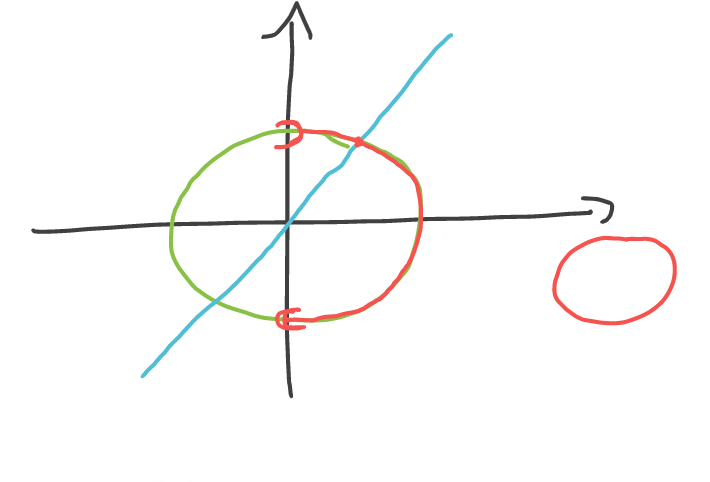
\includegraphics[width=0.5\linewidth]{projektion_r_2_beispiel}
    \caption*{\( \projectivedim{\projectionspace{V}}=1 \).}
    \label{fig:projektion_r_2_beispiel}
  \end{figure}
\end{beispiel*}
\begin{bemerkung*}
  Für \( V=\zeroset \) erhalte
  \begin{equation*}
    \projectivedim{\projectionspace{V}}=\dim{K}{f{V}}-1=0-1=-1
  \end{equation*}
  und \( \projectionspace{V}=\emptyset \).
\end{bemerkung*}
\begin{bspdef}
  Sei \( K \) ein Körper, \( n\geq 0 \). Dann ist \( \projectionspace{K^{n+1}} \) die Menge der Geraden durch den Ursprung im \( K^{n+1} \). Wir bezeichnen
  \begin{equation*}
    \projectionspaceover{n}{K}\definedas \projectionspace{K^{n+1}}
  \end{equation*}
  als \( n \)-dimensionalen projektiven Raum über \( K \).
\end{bspdef}
\begin{bemerkung*}
  Für einen \( K \)-Vektorraum \( V \) haben wir immer eine Abbildung
  \begin{equation*}
    \begin{split}
      V\setminus\zeroset &\to \projectionspace{V}\\
      v&\mapsto K\cdot v.
    \end{split}
  \end{equation*}
  \begin{figure}[H]
    \centering
    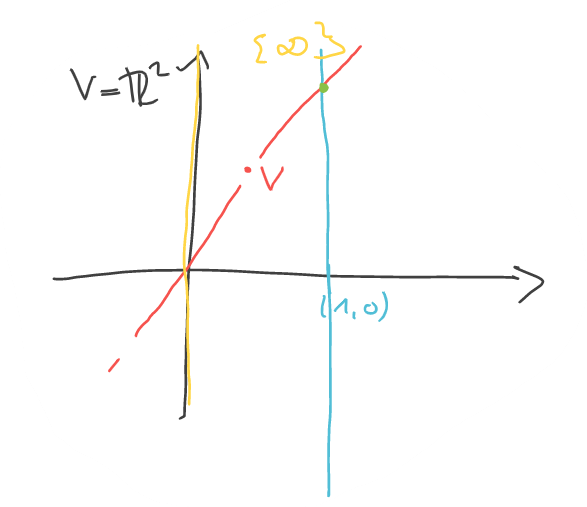
\includegraphics[width=0.5\linewidth]{einfachste_projektion}
    \caption*{\textcolor{Cyan}{\( \projectionspace{\reals^2}\text{\enquote{\( \sim \)}}\reals^1\cup \Set{\infty} \)}}
    \label{fig:einfachste_projektion}
  \end{figure}
\end{bemerkung*}
\begin{definition*}[homogene Koordinaten]
  \( n\in \logicspace _{\geq 0} \). Sei \( K \) ein Körper und \( L\in \projectionspaceover{n}{K} \). Wir nennen ein Tupel
  \begin{equation*}
    (x_0,\dots,x_n)\in K^{n+1}\setminus\zeroset
  \end{equation*}
  homogene Koordinaten des Punktes \( L\in \projectionspaceover{n}{K} \), falls 
  \begin{equation*}
    K\cdot (x_0,\dotsc,x_n)=L.
  \end{equation*}
  Schreibe auch
  \begin{equation*}
    (x_0:\dotsc:x_n)\definedas K\cdot(x_0,\dotsc,x_n).
  \end{equation*}
\end{definition*}
\begin{bemerkung*}
  Die homogenen Koordinaten eines Punktes \( L\in \projectionspaceover{n}{K} \) sind nur bis auf Multiplikation mit \( \lambda\in \fieldwithoutzero{K} \) eindeutig bestimmt, \dh für \( (x_0,\dotsc,x_n),(y_0,\dotsc,y_n)\in K^{n+1}\setminus \zeroset \) gilt
  \begin{equation*}
    (x_0:\dotsc:x_n)=(y_0:\dotsc:y_n)
  \end{equation*}
  \gdw
  \begin{equation*}
    K(x_0,\dotsc,x_n)=K(y_0,\dotsc,y_n),
  \end{equation*}
  \dh wenn \texists  \( \lambda\in \fieldwithoutzero{K} \) mit
  \begin{equation*}
    (x_0,\dotsc,x_n)=\lambda (y_0,\dotsc,y_n).
  \end{equation*}
\end{bemerkung*}
\section*{Unterräume eines projektiven Raums}
\begin{beispiel}\label{projektive_unterebene}
  \( V=\reals^3 \), die Menge der Geraden \( \reals\cdot(0,v_1,v_2) \) mit \( (v_1,v_2)\in \reals^2\setminus\zeroset \) \enquote{sieht genauso aus} wie
  \begin{equation*}
    \projectionspaceover{1}{\reals}=\projectionspace{\reals^2}.
  \end{equation*}
  Wir wollen
  \begin{equation*}
    \Set{\reals\cdot (0,v_1,v_2)|(v_1,v_2)\in \reals^2\setminus\zeroset\subseteq \projectionspace{\reals^3}}
  \end{equation*}
  als projektiven Unterraum erklären.
  \begin{figure}[H]
    \centering
    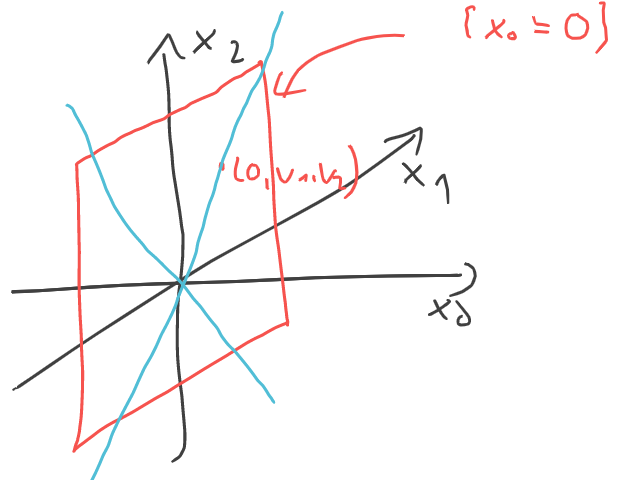
\includegraphics[width=0.5\linewidth]{projektiver_unterraum_beispiel}
    \label{fig:projektiver_unterraum_beispiel}
  \end{figure}
\end{beispiel}
\begin{definition*}
  Sei \( V \) ein \( K \)-Vektorraum und \( Z\subseteq \projectionspace{V} \). Wir nennen \( Z \) einen projektiven Unterraum von \( \projectionspace{V} \), falls es einen \( K \)-Untervektorraum \( W\untervektorraum V \) gibt mit \( Z=\projectionspace{W} \). Wir nennen \( Z\subseteq \projectionspace{V} \) eine
  \begin{itemize}
    \item (projektive) Gerade, wenn \( \projectivedim-{Z}=1 \),
    \item (projektive) Ebene, wenn  \( \projectivedim-{Z}=2 \),
    \item (projektive) Hyperebene, wenn \( \projectivedim-{Z}=\projectivedim{\projectionspace{V}}-1 \).
  \end{itemize}
\end{definition*}
\begin{bemerkung*}
  Ist \( Z\subseteq \projectionspace{V} \) ein projektiver Unterraum mit \( Z=\projectionspace{W} \) für einen Untervektorraum \( W\untervektorraum V\), so ist
  \begin{equation*}
    W=\bigcup_{p\in Z} p
  \end{equation*}
  Vereinigung von Geraden in \( Z \).
\end{bemerkung*}
Zurück zum obigen Beispiel: \( V=\reals^3 \), \( W=\Set{(0,x_1,x_2)|x_1,x_2\in\reals^3}\simeqq \reals^2 \). Dann ist \( Z=\projectionspace{W}\subseteq \projectionspace{V} \) ein projektiver Unterraum. Was bleibt übrig, wenn wir \( \projectionspace{\reals^3}\setminus\projectionspace{W} \) betrachten?
\begin{figure}[H]
  \centering
  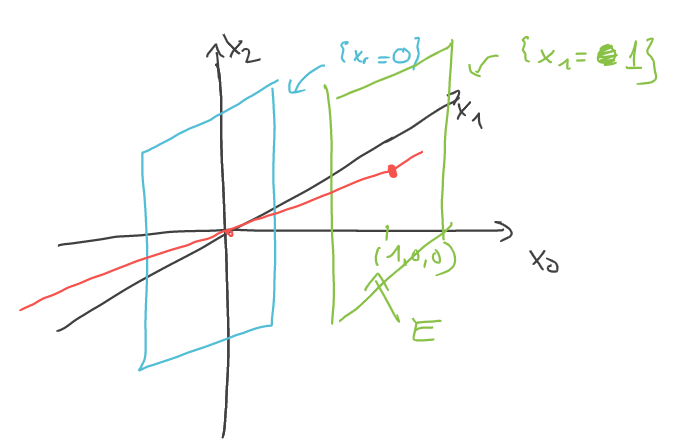
\includegraphics[width=0.5\linewidth]{ohne_projektiven_unterraum_r_2_beispiel}
  \label{fig:ohne_projektiven_unterraum_r_2_beispiel}
\end{figure}
\( \projectionspace{W} \): Geraden, die in der \( x_1 \)-\( x_2 \)-Ebene enthalten sind. Betrachte die affine Ebene
\begin{equation*}
  E=\Set{(1,x_1,x_2)|x_1,x_2\in \reals^2}\subseteq \reals^3.
\end{equation*}
Sei \( L\in \projectionspace{V}\setminus \projectionspace{W} \). Dann gibt es genau einen Schnittpunkt \( L\cap E \). Die Abbildung
\begin{equation*}
  \begin{split}
    \projectionspace{V}\setminus\projectionspace{W}&\to E\explain{\text{als affiner Raum über \( \reals \)}}{\simeqq}\reals^2\\
    L&\mapsto L\cap E
  \end{split}
\end{equation*}
ist bijektiv.

\minisec{Allgemein:} Sei \( K \) ein Körper und betrachte im \( K^{n+1} \) den Untervektorraum
\begin{equation*}
  W\definedas \Set{(x_0,\dotsc,x_n)\in K^{n+1}|x_0=0}.
\end{equation*}
Dann ist \( H\definedas \projectionspace{W}\subseteq \projectionspaceover{n}{K} \) eine (projektive) Hyperebene. Falls 
\begin{equation*}
  (y_0:\dotsc:y_n)\in \projectionspaceover{n}{K}\setminus H,
\end{equation*}
dann ist \( y_0\neq 0 \), also ist 
\begin{equation*}
  (y_0:\dotsc:y_n)=\left( 1:\frac{y_1}{y_0}:\dotsc:\frac{y_n}{y_0} \right)
\end{equation*}
von der Form \( (1:x_1:\dotsc:x_n) \) mit \( x_1,\dotsc,x_n \in K\). Zwei Tupel \( (x_1,\dotsc,x_n)\neq(x_1',\dotsc,x_n')\in K^n \) induzieren unterschiedliche Projektive Punkte im \( \projectionspaceover{n}{K} \).
\begin{equation*}
  (1:x_1:\dotsc:x_n)\neq (1:x_1':\dotsc:x_n')\in \projectionspaceover{n}{K}.
\end{equation*}
Aus
\begin{equation*}
  (1,x_1,\dotsc,x_n)=\lambda(1,x_1',\dotsc,x_n')
\end{equation*}
folgt \( \lambda=1 \).

Wir erhalten eine Bijektion
\begin{equation*}
  \begin{split}
    \phi\maps K^n&\to \projectionspaceover{n}{K}\setminus H\\
    (x_1,\dotsc,x_n)&\mapsto (1:x_1:\dotsc:x_n)
  \end{split}
\end{equation*}
und damit eine Einbettung
\begin{equation*}
  \begin{split}
    \iota\maps K^n&\to \projectionspaceover{n}{K}\\
    (x_1,\dotsc,x_n)&\mapsto (1:x_1:\dotsc:x_n),
  \end{split}
\end{equation*}
die wir kanonische Einbettung des \( K^n \) in den \( \projectionspaceover{n}{K} \) nennen.

\section*{Dimensionsformel als nächstes Ziel}
\begin{lemma}\label{schnitt_von_projektiven_unterraeumen_ist_projektiver_unterraum}
  Sei \( V \) ein \( K \)-Vektorraum und \( (Z_i)_{i\in I} \) eine Familie projektiver Unterräume von \( \projectionspace{V} \), \( i\in I \) gibt es eine Familie projektiver Unterräume von \( \projectionspace{V} \). Dann ist \( \bigcap_{i\in I} Z_i \) in projektiver Unterraum von \( \projectionspace{V} \).
\end{lemma}
\begin{proof}
  Zu jedem \( Z_i\subseteq \projectionspace{V} \), \( i\in I \), gibt es einen \( K \)-Untervektorraum \( W_i\subseteq V \) mit \( Z_i=\projectionspace{W_i} \). Es gilt
  \begin{equation*}
    \begin{split}
      \bigcap_{i\in I}Z_i&=\bigcap_{i\in I}\Set{L\subseteq V|\text{Gerade mit \( L\subseteq W_i \)}}\\
      &=\bigcap_{i\in I}\Set{L\subseteq V|\text{Gerade \( L \) mit \( L\subseteq  \smash{\underbrace{\bigcap_{i\in I}W_i}_{\mathclap{\text{\( K \)-Untervektorraum}}}\vphantom{\bigcup_{i\in I}}}\)}}\\
      &=\projectionspace*{\bigcap_{i\in I} W_i}
    \end{split}
  \end{equation*}
\end{proof}
\addtocounter{beispiel}{-1}
\begin{beispiel}
  \( V=\reals^3 \), also \( \projectionspace{V}=\projectionspaceover{2}{\reals} \) die projektive Ebene über \( \reals \).
  \begin{equation*}
    \begin{split}
      \iota\maps \reals^2&\to \projectionspaceover{2}{\reals}\\
      (x_1,x_2)&\mapsto (1:x_1:x_2)
    \end{split}
  \end{equation*}
  kanonische Einbettung. Betrachte die projektiven Geraden
  \begin{equation*}
    Z_1=\Set{(x_0:x_1:x_2)\in \projectionspaceover{2}{\reals}|x_1=0}=\projectionspace{W_1}
  \end{equation*}
  mit
  \begin{equation*}
    W_1=\Set{(x_0,x_1,x_2)\in\reals^3|x_1=0}
  \end{equation*}
  und \( Z_2=\projectionspace{W_2} \) it
  \begin{equation*}
    W_2=\Set{(x_0,x_1,x_2)\in \reals^3|x_0=x_1}.
  \end{equation*}
  Seien \( Y_1,Y_2\subseteq \reals^2 \) die affinen Geraden gegeben durch
  \begin{align*}
    Y_1&=\Set{(x_1,x_2)\in\reals^2|x_1=0}\\
    Y_2&=\Set{(x_1,x_2)\in \reals^2|x_1=1}.
  \end{align*}
  Dann ist \( Z_1=\iota(Y_1)\cup \Set{(0:0:1)} \) und \( Z_2=\iota(Y_2)\cup \Set{(0:0:1)} \). Es ist \( Y_1\cap Y_2=\emptyset \). (\( Y_1,Y_2 \) sind parallele Geraden), aber \( Z_1\cap Z_2=\Set{(0:0:1)} \). \enquote{Wir sagen auch, die Geraden \( Z_1,Z_2 \) schneiden sich in dem unendlich fernen Punkt \( (0:0:1) \)}.
  \begin{figure}[H]
    \centering
    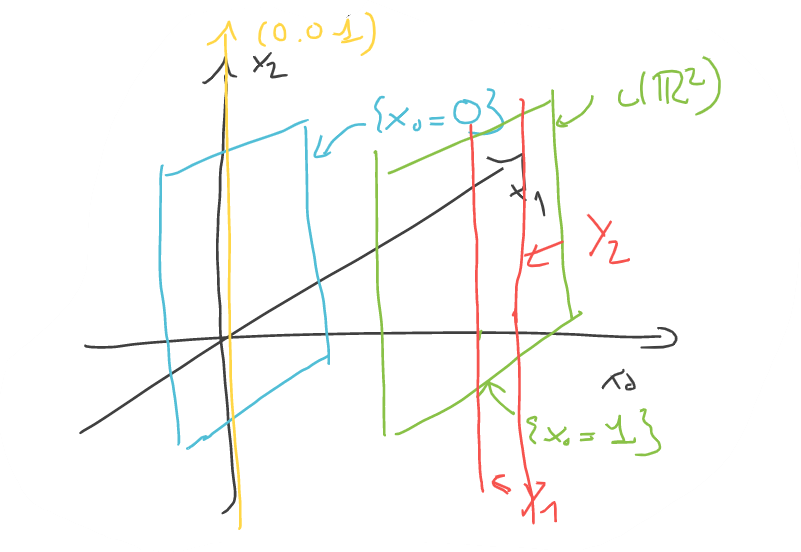
\includegraphics[width=0.5\linewidth]{schnitt_projektiver_geraden_r_3_beispiel}
    \label{fig:schnitt_projektiver_geraden_r_3_beispiel}
  \end{figure}
\end{beispiel}
\begin{bemerkung*}
  Die Vereinigung von projektiven Unterräumen eines projektiven Raumes \( \projectivedim{V} \) ist im Allgemeinen selbst kein projektiver Unterraum.
\end{bemerkung*}
\begin{frage*}
  Seien \( Z_i \), \( i\in I \) projektive Unterräume von \( \projectionspace{V} \). Finde den kleinsten projektiven Unterraum von \( \projectionspace{V} \), der \( \bigcup_{i\in I}Z_i \) enthält.
\end{frage*}
\begin{definition*}
  Sei \( V \) ein \( K \)-Vektorraum mit \( Z_i \), \( i\in I \) projektive Unterräume von \( \projectionspace{V} \). Wir definieren den Verbindungraum
  \begin{equation*}
    \bigvee_{i\in I}Z_i\definedas \bigcap_{\mathclap{\substack{Y\subseteq \projectionspace{V}\\
    \text{proj.\ Unterraum}\\
    \bigcup_{i\in I}Z_i\subseteq Y}}}Y.
  \end{equation*}
\end{definition*}
\begin{bemerkung*}
  \( \bigvee_{i\in I}Z_i \) ist der kleinste projektive Unterraum \( Y \) von \( \projectionspace{V} \) mit \( \bigcup_{i\in I}Z_i\subseteq Y \).
\end{bemerkung*}
\begin{lemma}\label{projektiver_verbindungsraum_formel}
  Sei \( V \) ein \( K \)-Vektorraum und \( W_i \), \( i\in I \) Untervektorräume von \( V \). Dann gilt
  \begin{equation*}
    \bigvee_{i\in I}\projectionspace{W_i}=\projectionspace*{\sum_{i\in I} W_i}.
  \end{equation*}
\end{lemma}
\begin{proof}
  Es ist 
  \begin{equation*}
    \bigcup_{i\in I} \projectionspace{W_i}\subseteq \projectionspace*{\sum_{i\in I}W_i}.
  \end{equation*}
  Sei \( Y=\projectionspace{W}  \) ein projektiver Unterraum mit
  \begin{equation*}
    \bigcup_{i\in I} \projectionspace{W_i}\subseteq Y
  \end{equation*}
  wobei \( W\subseteq V \) ein \( K \)-Untervektorraum ist. Dann gilt
  \begin{equation*}
    W_i=\bigcup_{\mathclap{p\in \projectionspace{W_i}}}p\subseteq \bigcup_{p\in Y}p=W,
  \end{equation*}
  also \( W_i\subseteq W \quad \forall i\in I\). \( W \) ist \( K \)-Untervektorraum, also gilt dann auch \( \sum_{i\in I}W_i\subseteq  W\) und
  \begin{equation*}
    \braceannotate{\supseteq\projectionspace{W_i}}{\projectionspace{\sum_{i\in I}W_i}}\subseteq \projectionspace{W}.
  \end{equation*}
\end{proof}